%---------------------------------------------------
% کلاس سند: article برای اسناد متنی، با اندازه کاغذ A4 و فونت پایه 16
\documentclass[a4paper,16pt]{article}

% بسته‌های ریاضی برای معادلات و نمادهای پیشرفته
\usepackage{amsmath, amssymb, amstext}

% بسته رنگ برای استفاده از رنگ در متن یا محیط‌ها
\usepackage{xcolor}

% بسته گرافیک برای درج تصاویر
\usepackage{graphicx}

% تنظیمات حاشیه صفحه
\usepackage{geometry}

% بسته لینک‌دهی (هایپرلینک‌ها)
\usepackage{hyperref}

% بسته صفحه‌آرایی برای تنظیم هدر و فوتر
\usepackage{fancyhdr}


% بسته xepersian برای پشتیبانی از زبان فارسی با XeLaTeX
\usepackage{xepersian}

% تعیین فونت فارسی (فایل فونت باید موجود باشد یا در سیستم نصب باشد)
\settextfont{B Nazanin}

% تنظیم اندازه حاشیه‌ها از هر طرف برابر با 1 اینچ
\geometry{margin=1in}

% تنظیم سبک fancy برای سربرگ و پاورقی
\pagestyle{fancy}

% سمت چپ هدر: مشخص‌کننده سری تمرین و نام درس
\lhead{تمرین سری دو درس فیزیک\lr{II }}

% وسط هدر: نام دانشکده
\chead{دانشکده فیزیک دانشگاه صنعتی خواجه نصیرالدین طوسی}

% سمت راست هدر: تاریخ روز به‌صورت خودکار
\rhead{\today}

% پایین صفحه: شماره صفحه
\cfoot{\thepage}

% شروع سند
\begin{document}
	
	% صفحه عنوان (بدون هدر و فوتر)
	\thispagestyle{empty}
	\begin{center}
		% لوگوی دانشگاه (باید فایل تصویر در مسیر پروژه باشد)
		
		
\includegraphics[width=0.5\textwidth]{../../../images/image-E_2/image-1.png} \\[10pt] 
		% عنوان سند
		\textbf{\LARGE عنوان:تمرین سری دو }\\[20pt]
		
		% نیم‌سال تحصیلی
		\textbf{\LARGE نیم‌سال تحصیلی:4032 }\\[10pt]
		
		% نام مدرس درس
		\textbf{\Large مدرس: ‫دكتر‬ ‫رضا‬ ‫افضل‬ ‫زاده‬}\\[10pt]
		
		% مبحث تمرین 
		\textbf{\Large ‫مبحث ‬‫تمرين‪:‬‬ ‫قانون‬ ‫گاوس‪،‬‬ ‫ميدان‬ ‫الكتريكي‬ }\\[10pt]
		
		% مهلت تحویل تمرین
		\textbf{\Large مهلت تحویل:۳۱ فروردین }
	\end{center}
	
	% صفحه جدید برای ادامه سند
	\newpage
	
	% ایجاد فهرست مطالب به‌صورت خودکار (براساس \section و \subsection و ...)
	\tableofcontents
	\newpage
	
	
	\section{سوال اول}
	‫‪.‬با‬‫استفاده‬ ‫از‬ ‫قانون‬ ‫گاوس‬ ‫ميدان‬ ‫الكتريكي‬ ‫را‬ ‫براي‬ ‫داخل‬ ‫و‬ ‫بيرون‬ ‫يك‬ ‫كره‬ ‫بدست‬ ‫اوريد‬
	\section{سوال دوم}
	يك گوي كوچك و غيررسانا با جرم
	\[
	m = 1.0~\mathrm{g}
	\]
	و بار الكتريكي
	\[
	q = 2.0 \times 10^{-8}~\mathrm{C}
	\]
	(كه به طور يكنواخت در حجم آن توزيع شده است)
	از يك نخ عايق اويزان است.
	اين نخ با يك صفحه غيررساناي باردار كه به صورت يكنواخت شارژ شده است،
	زاويه
	\[
	\theta = 30^\circ
	\]
	مي سازد
	(شكل به صورت مقطع نگاري نمايش داده شده است).
	
	با در نظر گرفتن نيروي گرانش وارد بر گوي و با فرض اينكه صفحه
	به طور بي نهايت در راستاي عمودي و به داخل و خارج از صفحه امتداد دارد،
	چگالي سطحي بار $\sigma$ صفحه را محاسبه كنيد.
	\begin{center}
		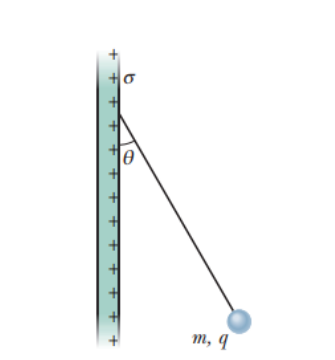
\includegraphics[width=0.5\textwidth]{../../../images/image-E_2/image-2.png} \\[10pt] 
	\end{center}
	
	\section{سوال سوم}
	يك توزيع بار كه از نظر كروي متقارن است اما از لحاظ شعاعي يكنواخت نيست،
	ميدان الكتريكي اي با بزرگي
	\[
	E = K r
	\]
	توليد مي كند كه به صورت شعاعي از مركز كره به سمت خارج هدايت مي شود.
	در اينجا $r$ فاصله شعاعي از مركز كره و $K$ يك ثابت است.
	
	چگالي حجمي بار $\rho(r)$ اين توزيع بار را محاسبه كنيد.
	
	\section{سوال چهارم}يك كره جامد غيررسانا داراي چگالي بار حجمي يكنواخت $\rho$ است.
	بردار $\vec{r}$ را از مركز كره به يك نقطه عمومي $P$ درون كره در نظر بگيريد.
	
	نشان دهيد كه ميدان الكتريكي در نقطه $P$ برابر است با
	\[
	\vec{E} = \frac{\rho}{3\varepsilon_0}\,\vec{r}
	\]
	
	(توجه كنيد كه اين نتيجه مستقل از شعاع كره است.)
	\section{سوال پنجم}
	بار به طور يكنواخت در كل حجم يك استوانه جامد با شعاع $R$
	و طول بي نهايت توزيع شده است.
	
	\begin{enumerate}
		\item[(الف)] نشان دهيد كه در فاصله $r < R$ از محور استوانه،
		ميدان الكتريكي برابر است با
		\[
		E(r) = \frac{\rho r}{2\varepsilon_0}
		\]
		كه در آن $\rho$ چگالي حجمي بار است.
		
		\item[(ب)] يك عبارت براي $E$ در حالتي كه $r > R$ است بنويسيد.
	\end{enumerate}
	\section{سوال ششم}
	در شكل زير، يك ميله نيمه بي نهايت غيررسانا
	(يعني در يك جهت بي نهايت است)
	داراي چگالي بار خطي يكنواخت $\lambda$ است.
	
	نشان دهيد كه بردار ميدان الكتريكي $\vec{E}$
	در نقطه $P$ با ميله زاويه
	45 درجه مي سازد و اين نتيجه مستقل از فاصله $R$ است.
		\begin{center}
		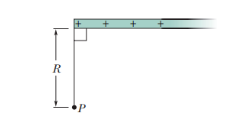
\includegraphics[width=0.5\textwidth]{../../../images/image-E_2/image-3.png} \\[10pt] 
	\end{center}
	\section{سوال هفتم}

ميدان الكتريكي روي محور يك حلقه باردار با شعاع $R$ به صورت زير بيان مي شود:
\[
E(z) = \frac{q z}{4 \pi \varepsilon_0 \left(R^2 + z^2\right)^{3/2}}
\]

فاصله اي از مركز حلقه كه در آن ميدان الكتريكي بيشينه مي شود، چقدر است؟
	\begin{center}
	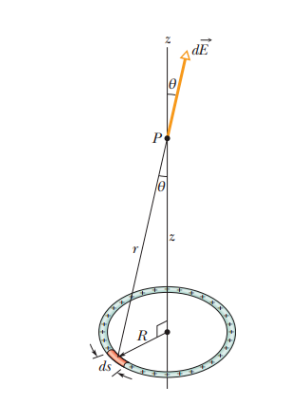
\includegraphics[width=0.5\textwidth]{../../../images/image-E_2/image-4.png} \\[10pt] 
\end{center}
	\section{سوال امتیازی}
	
	‫دو بار نقطه اي برابر با $q$ در فاصله $2a$ از يكديگر ثابت نگه داشته شده اند.
	يك بار نقطه اي آزمايشي در صفحه اي عمود بر خط واصل بين اين دو بار
	و در ميانه اين خط قرار دارد.
	
	فاصله اي را بيابيد كه در آن نيروي وارد بر بار آزمايشي بيشينه باشد.
	\\
	
	\textbf{موفق باشید.}
\end{document}
